\chapter{ارزیابی و بررسی}
در فصل قبل مشاهده کردیم که شبیه‌سازی ترافیک با موفقیت اجرا شد. مشکل این دوقلوی دیجیتال، دقت نسبتا پایین آن است. به طور مثال، بیشتر اوقات می‌توان لرزش و حرکت ریز خودرو‌های پارک شده را مشاهده کرد که نتیجه یکسان نبودن کادر محصورکننده این جسم، در طول فریم‌های مختلف است. همچنین در \cref{fig:DT_False_Positive} می‌توان مشاهده کرد که در پایین ماشین‌های پارک شده، ماشین دیگری نیز وجود دارد که در واقع متشکل از چهار موتور پارک‌ شده است. این نشان می‌دهد که تشخیص‌دهنده، خیلی اوقات ممکن است مثبت کاذب داشته باشد و یا به اشتباه طبقه‌بندی کند. پس با این حساب، نمی‌توان به مقدار ماشین‌هایی که در نیم ساعت تشخیص داده شده‌اند، اطمینان کرد. 

\begin{figure}[h!]
    \centering
    \begin{minipage}{0.8\textwidth}
        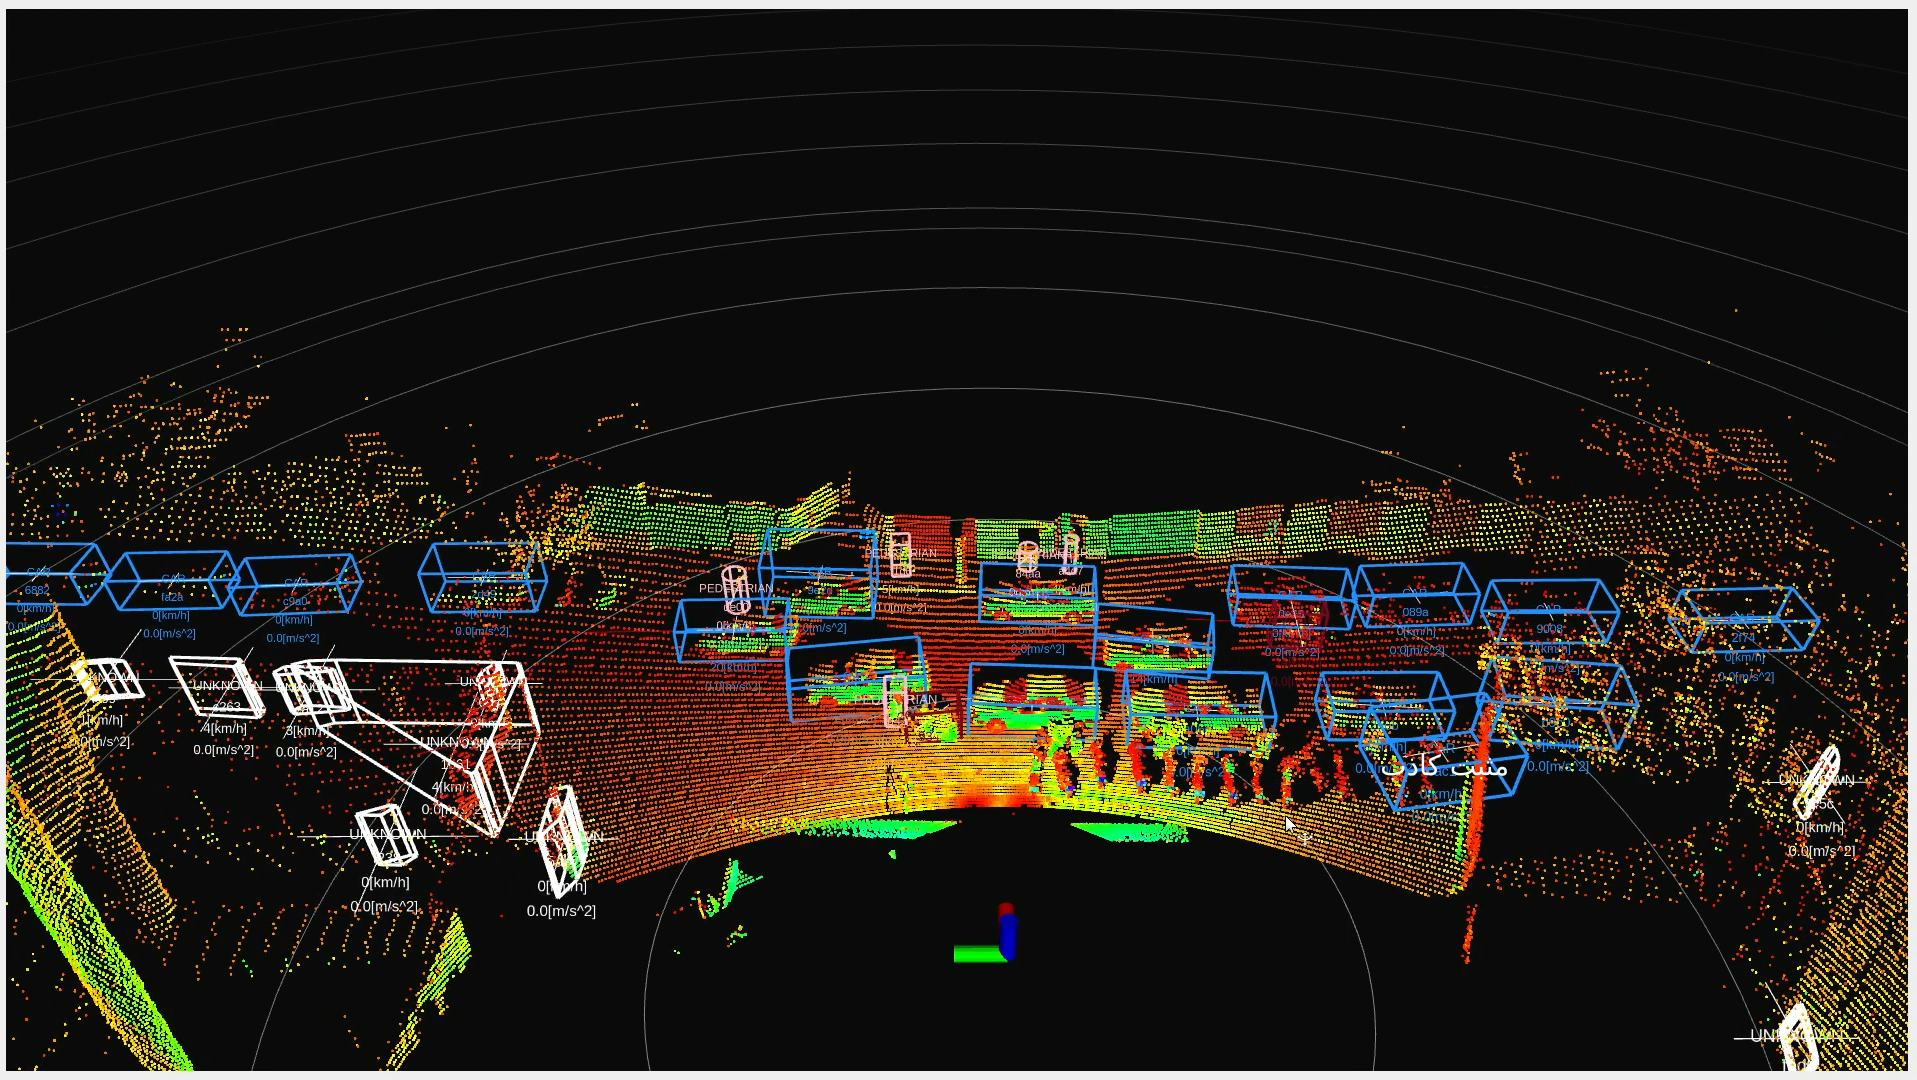
\includegraphics[width=1\linewidth]{figures/3D_Detection_FP.png}
    \end{minipage}
    \vspace{0.3cm}
    \begin{minipage}{0.8\textwidth}
        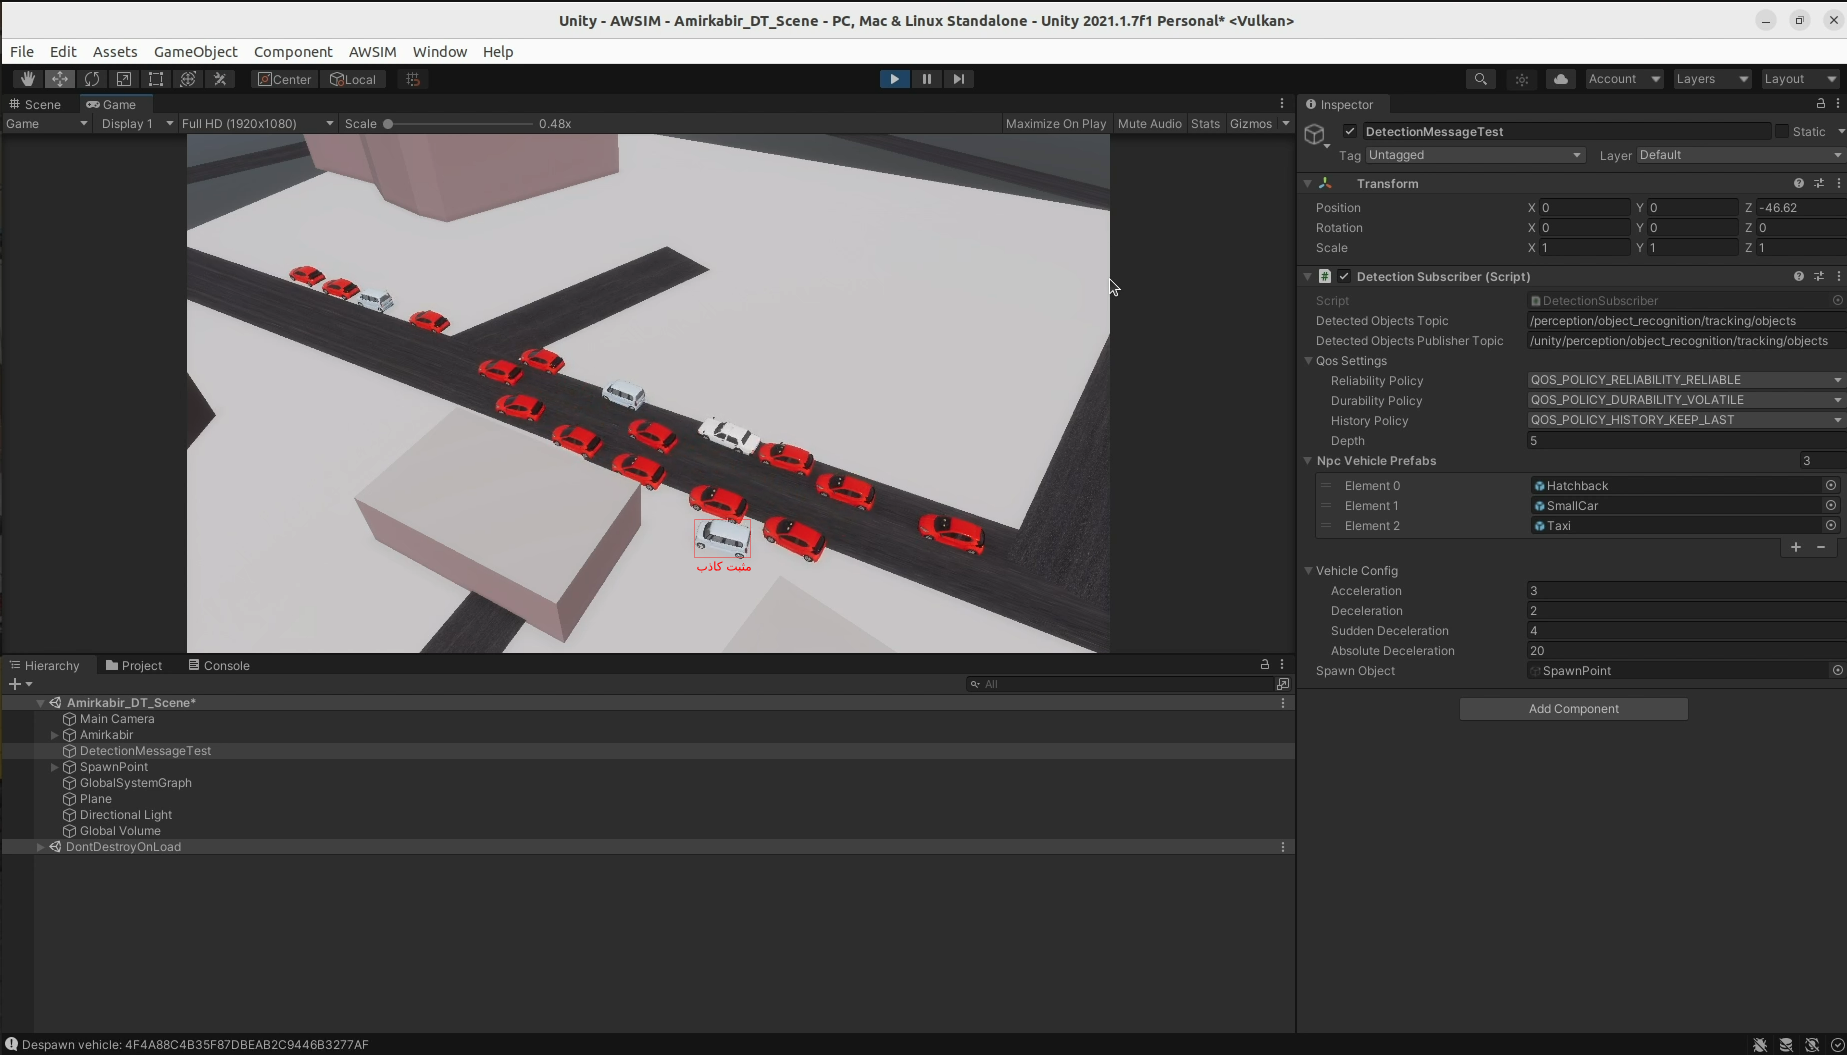
\includegraphics[width=1\linewidth]{figures/Amirkabir_DT_FP.png}
    \end{minipage}
    \caption{تصویری از مثبت کاذب تشخیص ‌داده شده}
    \label{fig:DT_False_Positive}
\end{figure}

در بخش دستکاری با فایل‌های اجرایی \lr{Autoware}، دو فیلتر مهم خاموش شده‌اند. این فیلتر‌ها باعث می‌شوند که تعداد مثبت‌ها کاذب کاهش یابد. به دلیل نداشتن نقشه ابر نقاط و نقشه برداری دقیق از منطقه دانشگاه صنعتی امیرکبیر، این فیلترها تا اطلاعات ثانویه خاموش خواهند بود. این بدین معنا است که مدل ردیاب هم‌زمان چند جسم ما، با داده‌هایی که مثبت‌های کاذب بیشتری دارد کار می‌کند و این موضوع از دقت آن می‌کاهد. به علت وجود نداشتن این فیلتر‌ها، برخی از اجسام متعلق به نقشه ابر‌ نقاط نیز، به اشتباه به عنوان اجسام حاضر در صحنه تشخیص داده می‌شوند.
\begin{figure}[h!]
    \centering
    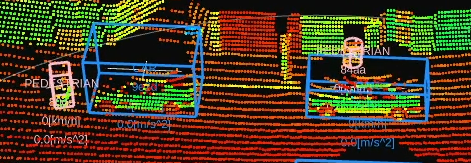
\includegraphics[width=1\linewidth]{figures/Pole_FP.png}
    \caption{تصویری از تشخیص اشتباه دو میله به عنوان عابرین پیاده}
    \label{fig:Pole_FP}
\end{figure}
همانطور که مشاهده می‌کنیم، \cref{fig:Pole_FP} این مشکل را به وضوح نمایش می‌دهد.

از دیگر مثبت‌های کاذب که می‌توان به آن اشاره کرد، تشخیص اشتباه موتور به عنوان عابر‌پیاده است. برای حل این مشکل راهی جز افزایش دقت مدل تشخیص‌دهنده و جستجو برای مدل‌های بهتر نداریم.
\cref{fig:DT_Occlusion_False_Positive}، تشخیص اشتباه موتورسیکلت را نمایش می‌دهد.\begin{figure}[h!]
    \centering
    \begin{minipage}{0.8\textwidth}
        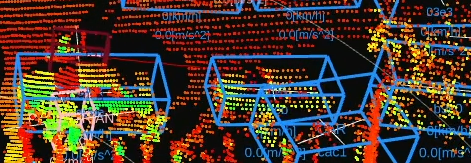
\includegraphics[width=1\linewidth]{figures/Motorbike_TP.png}
    \end{minipage}
    \vspace{0.3cm}
    \begin{minipage}{0.8\textwidth}
        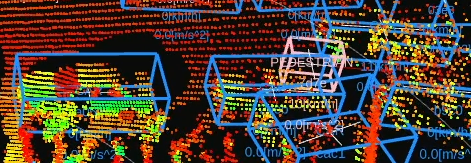
\includegraphics[width=1\linewidth]{figures/Motorbike_Occlusion_FP.png}
    \end{minipage}
    \caption{تصویری از تشخیص اشتباه موتوسیکلت به عنوان عابرپیاده}
    \label{fig:DT_Occlusion_False_Positive}
\end{figure} دلیل این تشخیص اشتباه، به موضوعی که در فصل دوم به آن پرداخته بر می‌گردد. این تشخیص اشتباه بخاطر اتفاقی به نام انسداد از بیرون یا \lr{External Occlusion} است. در این مثال، سیگنال‌های لایدار ماشین‌های پارک‌ شده، مانعی برای تشخیص موتورسیکلت به حساب می‌آیند.